\documentclass[%
autoref,     % тип документа
href,        % использовать пакет hyperref для создания гиперссылок
facsimile,   % отображать факсимиле диссертанта и ученого секретаря
colorlinks,  % цветные гиперссылки
%fixint,     % отключить прямые знаки интегралов
%times,      % шрифт Times как основной
%classified, % гриф секретности
]{disser}

\usepackage[
  a4paper, mag=1000,
  left=2.5cm, right=1cm, top=2cm, bottom=2cm, headsep=0.7cm, footskip=1cm
]{geometry}
\usepackage[T2A]{fontenc}
\usepackage[utf8]{inputenc}
\usepackage[english,russian]{babel}
\usepackage{tabularx}
\ifpdf\usepackage{epstopdf}\fi

\usepackage[style=gost-numeric,
  backend=biber,
  language=auto,
  hyperref=auto,
  autolang=other,
  defernumbers,
  sorting=none
]{biblatex}

\addbibresource{thesis.bib}

% Номера страниц снизу и по центру
%\pagestyle{footcenter}
%\chapterpagestyle{footcenter}

% Точка с запятой в качестве разделителя между номерами цитирований
%\setcitestyle{semicolon}

% Путь к файлам с иллюстрациями
\graphicspath{{fig/}}

\begin{document}
% Включение файла с общим текстом диссертации и автореферата
% (текст титульного листа и характеристика работы).
% ����� ���� ���������� ����� ����������� � ������������
\institution{�������� �����������}

\topic{���� �����������}

\author{��� ������}

\specnum{01.04.05}
\spec{������}
%\specsndnum{01.04.07}
%\specsnd{������ ����������������� ���������}

\sa{��� ������������}
\sastatus{�.~�.-�.~�., ����.}
%\sasnd{��� ������� ������������}
%\sasndstatus{�.~�.-�.~�., ����.}

%\scon{��� ������������}
%\sconstatus{�.~�.-�.~�., ����.}

\city{�����-���������}
\date{\number\year}

% ����� ������� ������������ � �����������
\mkcommonsect{actuality}{������������ ������}{%
����� �� ������������. ������~\cite{Yoffe_1993_AP_42_173}.
}

\mkcommonsect{objective}{���� ��������������� ������}{%
������� � ...

��� ���������� ������������ ����� ���� ������ ��������� ������:

}

\mkcommonsect{novelty}{������� �������}{%
����� � �������.
}

\mkcommonsect{value}{������������ ����������}{%
����������, ���������� � �����������, ����� ���� ������������ ��� ...
}

\mkcommonsect{results}{%
�� ������ ��������� ��������� �������� ���������� � ���������:}{%
����� � �����������.
}

\mkcommonsect{approbation}{��������� ������}{%
�������� ���������� ����������� ������������� �� ��������� ������������:
}

\mkcommonsect{pub}{����������.}{%
��������� ����������� ������������ � $N$ �������� �������, �� ��� $n_1$
������ � ������������� ��������~\citemy{Ivanov_1999_Journal_17_173,
Petrov_2001_Journal_23_12321,Sidorov_2002_Journal_32_1531}, $n_2$ ������ �
��������� ������ ����������� � $n_3$ ������� ��������.
}

\mkcommonsect{contrib}{������ ����� ������}{%
���������� ����������� � �������� ���������, ��������� �� ������, �������� ������������ ����� ������ � �������������� ������.
���������� � ���������� ���������� ����������� ����������� ��������� � ����������, ������ ����� ����������� ��� ������������. ��� �������������� � ����������� ���������� �������� ����� �������.
}

\mkcommonsect{struct}{��������� � ����� �����������}{%
����������� ������� �� ��������, ������ ����������, $n$ ����, ���������� � ������������.
����� ����� ����������� $P$ �������, �� ��� $p_1$ �������� ������, ������� $f$ ��������.
������������ �������� $B$ ������������ �� $p_2$ ���������.
}


% номер копии для грифа секретности
%\copynum{1}
% класс доступа
%\classlabel{Для служебного пользования}

\title{АВТОРЕФЕРАТ\\
диссертации на соискание ученой степени\\
доктора физико-математических наук}

\maketitle

% Внутренняя сторона обложки
\thispagestyle{empty}
\vspace*{-2cm}
\noindent
\begin{center}
Работа выполнена в \emph{название организации}.
\end{center}
\vskip1ex\noindent
\begin{tabularx}{\linewidth}{@{}lX@{}}
  \textbf{Научный консультант:} & \textbf{фамилия имя отчество}\\
  & ученая степень, ученое звание\\[6pt]
  \textbf{Официальные оппоненты:} & \textbf{фамилия имя отчество}\\
  & ученая степень, ученое звание\\[6pt]
  & \textbf{фамилия имя отчество}\\
  & ученая степень, ученое звание\\[6pt]
  & \textbf{фамилия имя отчество}\\
  & ученая степень, ученое звание\\[6pt]
  \textbf{Ведущая организация:} & название организации
\end{tabularx}

\vskip2ex\noindent
Защита состоится \datefield{} в \rule[0pt]{1cm}{0.5pt} часов
на заседании диссертационного совета \emph{шифр совета} при \emph{название
организации, при которой создан совет}, расположенном по адресу:
\emph{адрес}

\vskip1ex\noindent
С диссертацией можно ознакомиться в библиотеке
\emph{название организации}.

\vskip1ex\noindent
Автореферат разослан \datefield{}

\vskip2ex\noindent
Отзывы и замечания по автореферату в двух экземплярах, заверенные
печатью, просьба высылать по вышеуказанному адресу на имя ученого секретаря
диссертационного совета.

\vfill\noindent
\begin{minipage}[b]{0.4\linewidth}
  Ученый секретарь\\
  диссертационного совета,\\
  \emph{ученая степень}, \emph{ученое звание}
\end{minipage}
\hfill
% вставка файла, содержащего факсимиле ученого секретаря
\makeatletter
\ifDis@facsimile
  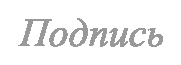
\includegraphics[width=3cm]{sec-facsimile}\hfill
\fi%
\makeatother%
\emph{фамилия и. о.}

\clearpage

\nsection{Общая характеристика работы}

% Актуальность работы
\actualitysection
\actualitytext

% Степень разработанности темы исследования
\developmentsection
\developmenttext

% Цели и задачи диссертационной работы
\objectivesection
\objectivetext

% Научная новизна
\noveltysection
\noveltytext

% Теоретическая и практическая значимость
\valuesection
\valuetext

% Методология и методы исследования
\methodssection
\methodstext

% Положения, выносимые на защиту
\resultssection
\resultstext

% Степень достоверности и апробация результатов
\approbationsection
\approbationtext

% Публикации
\pubsection
\pubtext

% Личный вклад автора
\contribsection
\contribtext

% Структура и объем диссертации
\structsection
\structtext

\nsection{Содержание работы}

\textbf{Во Введении} обоснована актуальность диссертационной работы, сформулирована цель и аргументирована научная новизна исследований, показана практическая значимость полученных результатов, представлены выносимые на защиту научные положения.

\textbf{В первой главе} ...

Содержание первой главы.

Результаты первой главы опубликованы в работе~\cite{Ivanov_1999_Journal_17_173}.

\textbf{Во второй главе} ...

Содержание второй главы.

Результаты второй главы опубликованы в работе~\cite{Petrov_2001_Journal_23_12321}.

\textbf{В третьей главе} ...

Содержание третьей главы.

Результаты третьей главы опубликованы в работе~\cite{Sidorov_2002_Journal_32_1531}.

\textbf{В Заключении}

% ----------------------------------------------------------------
\printbibliography[keyword=own,title={Основные публикации по теме диссертации}]
\printbibliography[notkeyword=own,title={Цитированная литература}]

% ----------------------------------------------------------------
% Выходные данные
\clearpage
\thispagestyle{empty}
\normalfont\selectfont
\vspace*{2cm}
\begin{center}
\textit{Научное издание}\\
\vskip 2cm
\makeatletter
\@author
\vskip 1.5cm
\@title{} на тему:\\
\@topic\\
\makeatother
\end{center}
\vfill
Подписано в печать~25.01.2011.
Формат~$60 \times 90$~1/16.
Тираж~100~экз.
Заказ~256.\\[2ex]
\noindent
Санкт-Петербургская издательская фирма <<Наука>> РАН.
199034, Санкт-Петербург, Менделеевская линия, 1,
\href{http://www.naukaspb.spb.ru}{http://www.naukaspb.spb.ru}

\end{document}
